\documentclass{article}
\usepackage{amsthm}
\usepackage{graphicx}
\usepackage{ctex}
\usepackage{amsmath}
\usepackage{amssymb} % 添加 amssymb 以支持更多符号
\usepackage{amsfonts}
\usepackage{tikz}
\usepackage{cancel}
\usepackage{listings}
\usetikzlibrary{arrows.meta} % 箭头样式
\usetikzlibrary{positioning} % 方便节点定位
\title{离散数学作业\_6}
\author{李云浩 241880324}
\date{\today}
\begin{document}
\maketitle
\section{6.1}
\subsection{T10}

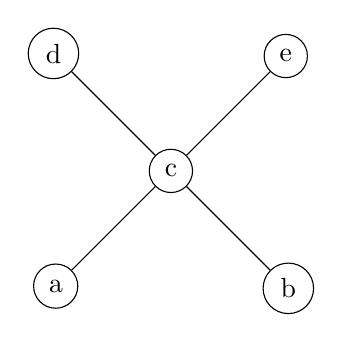
\begin{tikzpicture}[every node/.style={circle, draw}, node distance=1.5cm]
  \node (1) {c};
  \node (2) [below left=of 1] {a};
  \node (3) [below right=of 1] {b};
  \node (4) [above left=of 1] {d};
  \node (5) [above right=of 1] {e};
  
  \draw (1) -- (2);
  \draw (1) -- (3);
  \draw (1) -- (4);
  \draw (1) -- (5);
\end{tikzpicture}

\subsection{T13}
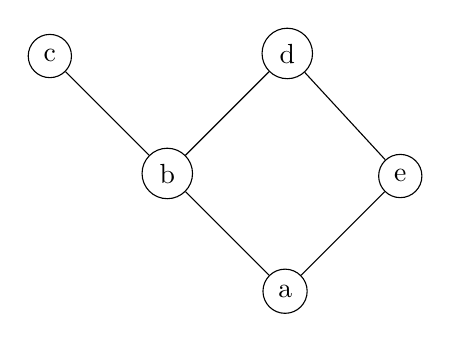
\begin{tikzpicture}[every node/.style={circle, draw}, node distance=1.5cm]
    \node (1) {a};
    \node (2) [above left=of 1]{b};
    \node (3) [above left=of 2]{c};
    \node (4) [above right=of 2]{d};
    \node (5) [above right=of 1]{e};
    \draw (1) -- (2);
    \draw (1) -- (5);
    \draw (2) -- (3);
    \draw (2) -- (4);
    \draw (5) -- (4);
\end{tikzpicture}
\subsection{T14}
\begin{tikzpicture}[every node/.style={circle, draw}, node distance=1.5cm]
    \node (1) {4};
    \node (2) [above=of 1]{3};
    \node (3) [above left=of 2] {2};
    \node (4) [above right=of 2]{5};
    \node (5) [above left=of 3]{1};
    
    \draw (1) -- (2);
    \draw (2) -- (3);
    \draw (2) -- (4);
    \draw (3) -- (5);
\end{tikzpicture}
\subsection{T16}
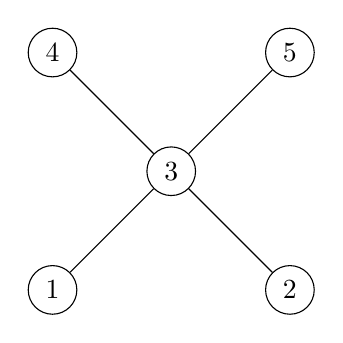
\begin{tikzpicture}[every node/.style={circle, draw}, node distance=1.5cm]
    \node (1) {3};
    \node (2) [below left=of 1] {1};
    \node (3) [below right=of 1] {2};
    \node (4) [above left=of 1] {4};
    \node (5) [above right=of 1] {5};
    
    \draw (1) -- (2);
    \draw (1) -- (3);
    \draw (1) -- (4);
    \draw (1) -- (5);
\end{tikzpicture}
  
\subsection{T18}
$
\begin{bmatrix}
    1 & 1 & 1 & 1 & 1\\
    0 & 1 & 0 & 1 & 0\\
    0 & 0 & 1 & 0 & 1\\
    0 & 0 & 0 & 1 & 0\\
    0 & 0 & 0 & 0 & 1
\end{bmatrix}
$
\subsection{T26}
(a) $\{\{1, 3, 12\}, \{2, 4\}\}$ \quad (b) $\{\{a, d, f\}, \{b, e\}, \{c\}\}$ \quad (c) $\{1, 2, 3, 4\}$\\
(d) $\{\{1, 3, 4, 6, 7, 8\}, \{2, 5\}\}$ \quad (e) $\{\{1, 2\}, \{3\}, \{4, 5, 6, 8, 9\}, \{7\}\}$
\subsection{T27}
(a) $\{2, 3\}$或$\{3, 4\}$ \quad (b) $\{a, b, c\}$ \quad (c) $\{1\}$
\quad (d) $\{2, 3\}$ \quad (e) $\{2, 3, 7, 8\}$
\subsection{T28}
相等。对于不可比的最大集合,因为该集合已经是最大的,因此其余所有图中的元素都至少与该集合中的任一元素有关系。
且因为剩余元素中不可比的最大数目小于等于最大集合内中的不可比元素数目。因此从该集合中的每个元素发散出一条链,必定可以
将其余所有元素连接起来。而每条链上的点都能组成具有全序的一个子集,且每条链之间必有一个点不相交。因此全序的子集个数与链的条数
以及最大不可比集合的基数相等。
\subsection{T29}
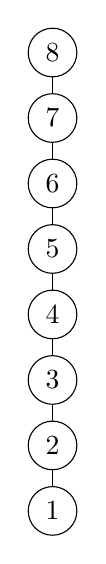
\begin{tikzpicture}[every node/.style={circle, draw}, node distance=0.2cm]
    \node (1) {1};
    \node (2) [above=of 1] {2};
    \node (3) [above=of 2] {3};
    \node (4) [above=of 3] {4};
    \node (5) [above=of 4] {5};
    \node (6) [above=of 5] {6};
    \node (7) [above=of 6] {7};
    \node (8) [above=of 7] {8};
    
    \draw (1) -- (2);
    \draw (2) -- (3);
    \draw (3) -- (4);
    \draw (4) -- (5);
    \draw (5) -- (6);
    \draw (6) -- (7);
    \draw (7) -- (8);
\end{tikzpicture}
  
\subsection{T30}
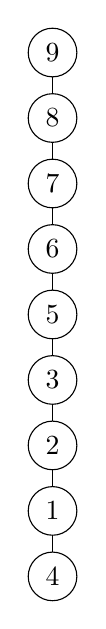
\begin{tikzpicture}[every node/.style={circle, draw}, node distance=0.2cm]
    \node (1) {4};
    \node (2) [above=of 1] {1};
    \node (3) [above=of 2] {2};
    \node (4) [above=of 3] {3};
    \node (5) [above=of 4] {5};
    \node (6) [above=of 5] {6};
    \node (7) [above=of 6] {7};
    \node (8) [above=of 7] {8};
    \node (9) [above=of 8] {9};
    \draw (1) -- (2);
    \draw (2) -- (3);
    \draw (3) -- (4);
    \draw (4) -- (5);
    \draw (5) -- (6);
    \draw (6) -- (7);
    \draw (7) -- (8);
    \draw (8) -- (9);
\end{tikzpicture}
\subsection{T34}
非自反性:$\forall a \in A$, $a < a$不成立,因此是非自反的。\\
传递性:$\forall a, b, c \in A$,当$a < b$且$b < c$时,显然有$a < c$。因此具有传递性。\\
综上所述,通常的关系$<$是$A$上的一个拟序。
\subsection{T35}
非自反性:因为$R$是$A$上的一个拟序,因此$\forall a \in A$,$(a, a) \notin R$。所以$(a, a) \notin R^{-1}$,因此是非自反的。\\
传递性:$\forall a, b, c(a, b, c \in A \land (a, b) \in R \land (b, c) \in R)$,有$(a, c) \in R$。
因此$\forall a, b, c(a, b, c \in A \land (b, a) \in R^{-1} \land (c, b) \in R^{-1})$,有$(c, a) \in R^{-1}$。因此$R^{-1}$具有传递性。\\
综上所述,$R^{-1}$也是$A$上的一个拟序。
\subsection{T36}
$R'$表示$\{(a, b) |\ a | b \land a \neq b\}$。\\
非自反性:由$R'$的定义可知,$\forall a, b$,如果$a = b$,显然$(a, b) \notin R'$,因此是非自反的。\\
传递性:因为整除本身具有传递性,故$R'$也具有传递性。\\
因此$R'$为$Z^+$上的一个拟序。
\subsection{T38}
自反性:对于任意二阶布尔矩阵$M$,一定有$m_{ij} = n_{ij}, 1\leq i \leq 2, 1 \leq j \leq 2$。因此$R$满足自反性。\\
反对称性:$\forall M, N \in A, M \neq N \land M R N$。则必定存在$m_{ij} < n_{ij}$。因此$n_{ij} > m_{ij}$,所以$(N, M) \notin R$,因此$R$满足反对称性。\\
传递性:因为运算$\leq$具有传递性,因此$\forall M, N, O \in A, (M, N) \in R \land (N, O) \in R$,即$\forall i, j (m_{ij} \leq n_{ij}) \land (n_{ij} \leq o_{ij}) \rightarrow (m_{ij} < o_{ij})$。
故$(M, O) \in R$,因此满足传递性。\\
综上所述,因为$R$满足自反性、反对称性、传递性,因此$R$是$A$上的一个偏序。
\subsection{T40}
对于$(A, \leq)$,因为$1 | 2 \land 2 | 4 \land 4 | 8$,因此$(A, \leq)$是一个全序关系。
对于$(A', \leq')$,因为$0 \leq 1 \leq 2 \leq 3$,所以$(A', \leq')$也是一个全序关系。
因为$(A, \leq),(A', \leq')$都是全序关系并且元素都为4个,因此必定同构。
\section{6.2}
\subsection{T6}
无极大元,极小元为0
\subsection{T8}
极小元$2, 3$\quad 极大元48
\subsection{T12}
最大元5,无最小元
\subsection{T14}
最小元0,最大元1
\subsection{T17}
不等价,在如下的哈斯图中,$2$是$A$的一个极大元,不存在$c \in A$使得$2 < c$。但是$\exists 3 \in A$,
$3 \leq 2$不成立。因此命题不等价。
$$
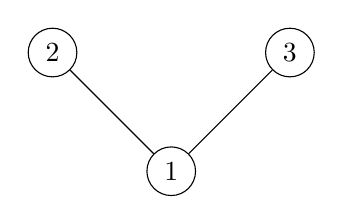
\begin{tikzpicture}[every node/.style={circle, draw}, node distance=1.5cm]
    \node (1) {1};
    \node (2) [above left=of 1] {2};
    \node (3) [above right=of 1] {3};
    
    \draw (1) -- (2);
    \draw (1) -- (3);
\end{tikzpicture}$$
\subsection{T18}
不等价,在如下的哈斯图中,$1$是$A$的一个极小元,不存在$c \in A$使得$c < 1$。
但是$\exists 2 \in A$, $1 \leq 2$不成立。因此命题不等价。
$$
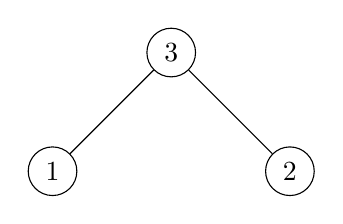
\begin{tikzpicture}[every node/.style={circle, draw}, node distance=1.5cm]
    \node (1) {3};
    \node (2) [below left=of 1] {1};
    \node (3) [below right=of 1] {2};
    
    \draw (1) -- (2);
    \draw (1) -- (3);
\end{tikzpicture}
$$
\subsection{T19}
(a) 真命题。在$A$中任取一个元素$a_0$,如果$\exists a_1 (a_1 \in A \land a_1 > a_0)$,
则换取$a_1$,重复上述过程。因为偏序集为有限集,因此必定$\exists a_k(a_k \in A \land \nexists a_i (a_i \in A \land a_i > a_k))$。
故必定存在$a_k$为极大元\\
(b) 假命题。参考17题的哈斯图,不存在最大元\\
(c) 真命题。在$A$中任取一个元素$a_0$,如果$\exists a_1 (a_1 \in A \land a_1 < a_0)$,
则换取$a_1$,重复上述过程。因为偏序集为有限集,因此必定$\exists a_k(a_k \in A \land \nexists a_i (a_i \in A \land a_i < a_k))$。
故必定存在$a_k$为极小元\\
(d) 假命题。参考18题的哈斯图,不存在最小元。
\subsection{T20}
假设存在两个最大元$a_1, a_2$。因为它们是最大元,因此有$\forall a \in A \rightarrow a \leq a_1 \land a \leq a_2$。因为$a_1 \in A \land a_2 \in A$。
因此$a_1 \leq a_2 \land a_2 \leq a_1 \rightarrow a_1 = a_2$,因此只有一个最大元
\subsection{T22}
设$B$的上界为集合$C$,$B$有两个最小上界$c_1, c_2$。因此有$\forall c \in C \rightarrow c_1 \leq c \land c_2 \leq c$。因为$c_1 \in C \land c_2 \in C$。
因此$c_1 \leq c_2 \land c_2 \leq c_1 \rightarrow c_1 = c_2$,因此至多只有一个最小上界。\\
同理可证,$B$至多只有一个最大下界。
\subsection{T23}
(a) $\{g, f, h\}$ \quad (b) $\{a, b, c\}$ \quad (c) $f$ \quad (d) $c$ 
\subsection{T24}
(a) $\varnothing$ \quad (b) $\varnothing$ \quad (c) 无 \quad (d) 无
\subsection{T25}
(a) $\{d, e, f\}$ \quad (b) $\{a, b\}$ \quad (c) $d$ \quad (d) $b$ 
\subsection{T26}
(a) $\{5\}$ \quad (b) $\{1, 2, 3\}$ \quad (c) $5$ \quad (d) $3$
\subsection{T32}
(a) $\left\{
    \begin{bmatrix}
        1 & 1\\
        0 & 1
    \end{bmatrix},
    \begin{bmatrix}
        1 & 1\\
        1 & 1
    \end{bmatrix}
\right\}$\quad
(b) $\left\{
    \begin{bmatrix}
        0 & 0\\
        0 & 0
    \end{bmatrix},
    \begin{bmatrix}
        0 & 0\\
        0 & 1
    \end{bmatrix}
\right\}$\quad
(c) $\begin{bmatrix}
    1 & 1\\
    0 & 1
\end{bmatrix}$\quad
(d) $\begin{bmatrix}
    0 & 0\\
    0 & 1
\end{bmatrix}$
\subsection{T33}
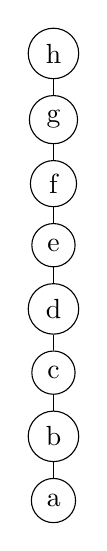
\begin{tikzpicture}[every node/.style={circle, draw}, node distance=0.2cm]
    \node (1) {a};
    \node (2) [above=of 1] {b};
    \node (3) [above=of 2] {c};
    \node (4) [above=of 3] {d};
    \node (5) [above=of 4] {e};
    \node (6) [above=of 5] {f};
    \node (7) [above=of 6] {g};
    \node (8) [above=of 7] {h};
    
    \draw (1) -- (2);
    \draw (2) -- (3);
    \draw (3) -- (4);
    \draw (4) -- (5);
    \draw (5) -- (6);
    \draw (6) -- (7);
    \draw (7) -- (8);
\end{tikzpicture}
\subsection{T35}
假设$a_1$为$A$的极大元,由极大元的定义可知:$\forall a(a \in A \rightarrow a \leq a_1)$因此$\forall a(a \in A \rightarrow (a, a_1) \in R)$。
因此在$M_R$,若存在第$a_k$列全为$1$,则$a_k$是$A$的最大元。\\
同理,在$M_R$中,若存在第$a_i$行全为$1$,则$a_i$是$A$的最小元。
\subsection{T36}
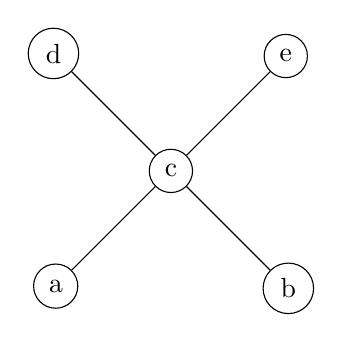
\begin{tikzpicture}[every node/.style={circle, draw}, node distance=1.5cm]
    \node (1) {c};
    \node (2) [below left=of 1] {a};
    \node (3) [below right=of 1] {b};
    \node (4) [above left=of 1] {d};
    \node (5) [above right=of 1] {e};
    
    \draw (1) -- (2);
    \draw (1) -- (3);
    \draw (1) -- (4);
    \draw (1) -- (5);
\end{tikzpicture}
\subsection{T37}
(a) 从$51 \sim 100$,$A$中都不存在它们除本身外的倍数。而从$2 \sim 50$,它们的2倍都在$A$中。因此$(A, \leq)$有50个极大元\\
(b) $\{2, 4, 8, 16, 32, 64\}$
\subsection{T38}
$(A, \leq)$中极小元的个数即从$2 \sim 100$中,质数的个数。因此极小元组成的集合。\\
为:$\{2, 3, 5, 7, 11, 13, 17, 19, 23, 29, 31, 37, 41, 43, 47, 53, 59, 61, 67, 71, 73, 79, 83, 89, 97\}$
共$25$个。
\section{6.3}
\subsection{T1}
对于该哈斯图中的任意两个元素,它们的最小上界和最大下界都在哈斯图中,是格。
\subsection{T2}
$e \lor f$以及$a \land b$不在哈斯图中,不是格。
\subsection{T3}
$e \land d$不在哈斯图中,不是格。
\subsection{T4}
对于该哈斯图中的任意两个元素,它们的最小上界和最大下界都在哈斯图中,是格。
\subsection{T5}
对于该哈斯图中的任意两个元素,它们的最小上界和最大下界都在哈斯图中,是格。
\subsection{T6}
对于该哈斯图中的任意两个元素,它们的最小上界和最大下界都在哈斯图中,是格。
\subsection{T13}
假设用$n$为的布尔代数来代替$S$中的元素,因为$T$是$S$的一个子集,$P(T)$即取$n - r$位固定为0,其余位数任意。
因此,对于$P(T)$,$\forall a, b \in P(T)$,$a$和$b$的$n - r$位同为0,取$\lor$或$\land$运算后,那$n - r$位仍为0。
因此$\forall a, b \in P(T) \rightarrow (a \land b) \in P(T), (a \lor b) \in P(T)$,故运算封闭。因此$P(T)$是$L$的一个子格。
\subsection{T14}
$\forall x, y \in [a, b]$,有$(a \leq x \leq b) \land (a \leq y \leq b)$。
因此$(a \leq (x \land y) \leq b) \land (a \leq (x \lor y) \leq b)$。因此$x, y$的上界和下界都在这个区间内。
因此区间$[a, b]$关于$\land,\lor$运算是闭合的。因此$[a, b]$是$L$的一个子格。
\subsection{T15}
对于全序偏序集,其中任意两个元素皆可比,因此其子集中的任意两个元素仍然是可比的,即其子集仍为一个全序偏序集。
显然对于一个全序偏序集,一定是关于$\land,\lor$闭合的。因此全序偏序集的子集是一个子格。
\subsection{T18}
反证法:假设$0 = I$,有$\forall x \in L, 0 \leq x \leq I \rightarrow 0$。
因此所有格中的元素都为$0$,则所有元素不具有偏序关系,则不属于一个格。
因此原假设不成立,即$0 \neq I$。
\subsection{T19}
充分性:$a \land b = a \rightarrow a \leq b$\\
因为$(a \land b) \leq b$,又因为$a = a \land b$,因此$a \leq b$。\\
必要性:$a \leq b \rightarrow (a \land b = a)$\\
因为$a \leq b$,因此$a \land b$是$a, b$的最大下界。同时$(a = a) \land (a \leq b)$,因此$a$也是
$a, b$的最大下界。因此$a \land b = a$。
\subsection{T20}
在$D_n$中,$a \land b = GCD(a, b), a \lor b = LCM(a, b)$。因此$a \lor (b \land c) = LCM(a, GCD(b, c))$。
$(a \lor b) \land (a \lor c) = GCD(LCM(a, b), LCM(a, c))$。而对于$\forall a, b, c \in N, LCM(a, GCD(b, c)) = GCD(LCM(a,b), LCM(a, c))$
成立,因此$a \lor (b \land c) = (a \lor b) \land (a \lor c)$也成立。故对于任意的$n$,$D_n$是分配的。
\subsection{T22}
对于分配格$A$,有:$\forall a_1, a_2, a_3 \in A \rightarrow (a_1 \lor (a_2 \land a_3) = (a_1 \lor a_2) \land (a_1 \lor a_3))$.
因此对于其子格$B$,关于$\land,\lor$运算闭合,有$\forall b_1, b_2, b_3 \in B \rightarrow b_1, b_2, b_3 \in A$。
因此$b_1 \lor (b_2 \land b_3) = (b_1 \lor b_2) \land (b_1 \lor b_3)$。因此$B$也是分配格。因此分配格的子格也是分配格。
\subsection{T24}
\begin{align*}
    a \lor (a' \land b) &= (a \lor a') \land (a \lor b)\\
    &= 1 \land (a \lor b)\\
    &= a \lor b
\end{align*}
\begin{align*}
    a \land (a' \lor b) &= (a \land a') \lor (a \land b)\\
    &= 0 \lor (a \land b)\\
    &= a \land b
\end{align*}
\subsection{T25}
\begin{align*}
    x &= x \land (a \lor x)\\
    &= x \land (a \lor y)\\
    &= (a \land x) \lor (x \land y)\\
    &= (a \land y) \lor (x \land y)
\end{align*}
\begin{align*}
    y &= y \land (a \lor y)\\
    &= y \land (a \lor x)\\
    &= (a \land y) \lor (x \land y)
\end{align*}
因此$x = (a \land y) \lor (x \land y) = y$,证毕。
\subsection{T26}
(a)因为$a \leq c \rightarrow a \lor c = c$,所以:
\begin{align*}
    a \lor (b \land c) &= (a \lor b) \land (a \lor c)\\
    &= (a \lor b) \land c
\end{align*}证毕。\\
(b) 右图为菱形格,不满足分配律。$a \land (b \lor c) = a \neq (a \land b) \lor (a \land c) = 0$。
并且讨论(1)当$c = I$时,$a \lor (b \land c) = a \lor b = (a \lor b) \land c$,成立。\\
(2)当$c = 0$时,$a = 0$。$a \lor (b \land c) = 0 = (a \lor b) \land c$。\\
(3)当$c = c$时,$a = 0$。$a \lor (b \land c) = b \land c = (a \lor b) \land c$\\
证毕,右图为一个非分配的模格。 
\subsection{T27}
$D_{42}$中的元素有$1, 2, 3, 6, 7, 14, 21, 42$。\\
其中$1 \sim 42, 2 \sim 21, 3 \sim 14, 6 \sim 7$,相互为各自的补。
\subsection{T29}
因为$a, b, c, d, e$部分与五边形格同构,因此不满足分配关系。\\
因为$c$不存在补元,因此也不满足补的关系。
\subsection{T34}
$a$的补是$e$。$b$的补是$c$,$c$的补是$b$或$d$,$d$的补是$c$,$e$的补是$a$。
\subsection{T37}
对于一个布尔代数格$00 \sim 11$,取其子格$\{11, 10, 00\}$,因此其子格中的$10$不具有补元,因此原命题不成立。
\subsection{T38}
取一个无限格$A$,元素为$[0, 1]$中的全体实数,关系取$\leq$。取其子格$(0, 1)$,那么子格将会是一个无界格。
因此原命题不成立。
\subsection{T39}
假设原格$A$是可模的,即$\forall a_1, a_2, a_3 \in A \rightarrow a_1 \lor (a_2 \land a_3) = (a_1 \lor a_2) \land a_3$。
取其子格$B$,对于$\forall b_1, b_2, b_3 \in B \rightarrow b_1, b_2, b_3 \in A$。因此$b_1 \lor (b_2 \land b_3) = (b_1 \lor b_2) \land b_3$。
因此一个模格的子格也是可模的。
\subsection{T40}
对于一个全序$A$,$\forall a_1, a_2, a_3 \in A$,不妨假设$a_1 < a_2 < a_3$。因此:
$$
    a_1 \lor (a_2 \land a_3) = a_1 \lor a_2 = a_2
$$
$$
    (a_1 \lor a_2) \land (a_1 \lor a_3) = a_2 \land a_3 = a_2
$$
因此:$a_1 \lor (a_2 \land a_3) = (a_1 \lor a_2) \land (a_1 \lor a_3)$。可进一步枚举,可证得全序满足分配律。
\end{document}
